\documentclass[a4paper, 12pt]{article}

\newcommand{\assignmentAuthor}{Bhaskar Goyal}
\newcommand{\course}{CSCI - 567}
\newcommand{\assignmentName}{HW 01}
\newcommand{\USCID}{6547367383}
\newcommand{\assignmentDate}{July 3, 2021}

\addtolength{\hoffset}{-2.25cm}
\addtolength{\textwidth}{4.5cm}
\addtolength{\voffset}{-2.5cm}
\addtolength{\textheight}{5cm}
\setlength{\parskip}{0pt}
\setlength{\parindent}{15pt}

\usepackage{amsthm}
\usepackage{amsmath}
\usepackage{amssymb}
\usepackage{bm}
\usepackage{tikz}
\usetikzlibrary{automata}
\usepackage{enumitem}
\usepackage{mathabx}
\usepackage{algorithmic}
\usepackage[colorlinks = true, linkcolor = black, citecolor = black, final]{hyperref}
\usepackage{tikz}
\usetikzlibrary{automata}

\usepackage{graphicx}
\usepackage{multicol}
\usepackage{ marvosym }
\usepackage{wasysym}
\usepackage{tikz}
\usetikzlibrary{patterns}
\usepackage{fancyhdr}
\usepackage{amssymb,latexsym,amsmath,amsthm}
\usepackage{amsfonts,rawfonts}
\usepackage{thmtools}
\usepackage{systeme}
\usepackage{mathtools}

\pagestyle{fancy}
\fancyhf{}
\rhead{\assignmentAuthor \; (USC ID - \USCID)}
\lhead{\course \; \assignmentName}
\rfoot{Page \thepage}
\lfoot{\assignmentDate}

\newcommand{\ds}{\displaystyle}

\setlength{\parindent}{0in}
\graphicspath{ {./images/} }

\declaretheoremstyle[
headfont=\color{blue}\normalfont\bfseries,
notefont=\bfseries, 
notebraces={}{},
% bodyfont=\color{red}\normalfont\itshape,
bodyfont=\normalfont,%\itshape,
%headformat=\NUMBER.~\NAME\NOTE
headformat=\NAME\NOTE
]{colorquestion}

\declaretheorem[
numbered=no,
style=colorquestion,
name=Question
]{question}

\title{\course \; \assignmentName}
\author{\textbf{\assignmentAuthor} \\ \Small{USC ID - \USCID}}
\date{\assignmentDate}

% ----------------------------

% The "stuff" above here is called the preamble of the document.  It sets the margins and loads special packages.  Probably the only reason you would need to edit something above here would be to add a package to do something very specific... but probably everything you need is loaded already

% -----------------------------

\begin{document}
\thispagestyle{plain}
\maketitle
\hrule
\bigskip

% -------------------------
% Question 1
% -------------------------

\begin{proof}[\color{red}{\textbf{Problem 1}: Name}]

\hfill

\begin{enumerate}[label={\color{blue}{\textbf{1.\arabic*})}}]
    \item 
        To calculate Test Error, we need to predict the test data points\\
        \textbf{Point 1:} $x_1 = 0.8, x_2 = 0.8, y = 0$ \\
        $y_{Predicted} = 0$ \\
        (Because, $x_1 > 0.5$ and $x_2 > 0.5$). \\
        $\therefore$ Point 1 is correctly classified. \\
        \textbf{Point 2:} $x_1 = 0.6, x_2 = 0.4, y = 1$ \\
        $y_{Predicted} = 1$ \\
        (Because, $x_1 > 0.5$ and $x_2 < 0.5$). \\
        $\therefore$ Point 2 is correctly classified. \\
        \textbf{Test Error}
        \begin{align*}
            \text{Test Error} &= \frac{\text{Misclassified Test Points}}{\text{Total Test Points}} \\
            &= \frac{0}{2} \\
            &= 0
        \end{align*} 
        Hence, the Test Error = 0
        
    \item 
        To calculate Test Error, we need to predict the test data points using the new Decision Tree from Figure 3 (in question). \\
        \textbf{Point 1:} $x_1 = 0.8, x_2 = 0.8, y = 0$ \\
        $y_{Predicted} = 1$ \\
        (Because, $x_1 > 0.5$). \\
        $\therefore$ Point 1 is misclassified. \\
        \textbf{Point 2:} $x_1 = 0.6, x_2 = 0.4, y = 1$ \\
        $y_{Predicted} = 1$ \\
        (Because, $x_1 > 0.5$. \\
        $\therefore$ Point 2 is correctly classified. \\
        \textbf{Test Error}
        \begin{align*}
            \text{Test Error} &= \frac{\text{Misclassified Test Points}}{\text{Total Test Points}} \\
            &= \frac{1}{2}
        \end{align*} 
        Hence, the Test Error = $1/2 = 0.5$
        
        
    \item 
        Yes, the decision tree in Figure 3 is a \textbf{linear} classifier in terms of $(x_1, x_2)$. This is because the condition on root node of decision tree is $x_1 > 0.5$ which is a linear equation in $x_1$.
        \smallskip
        
        No, we can't classify the given data in Table 1 and get zero classification error by drawing a depth-1 decision tree similar to Figure 3. This is because the data points are \textbf{non-linearly separable}. 
        
    
    \item
        Yes, because the data points are \textbf{non-linearly separable}, we can get zero classification error by putting any expression of variables like $f(x_1, x_2) \geq c$ or $f(x_1, x_2) \leq c$. \\
        This means, we can put a non-linear function equation which separate the data points into 2 distinct regions. \\
        Any elliptical or hyperbolic equation which separate the data points into 2 distinct regions will give zero error. \\
        Ex. Below is a ellipse equation which separate the data points. 
        \begin{align*}
            \frac{\left(\left(x-0.5\right)\cos\left(\frac{\pi}{4}\right)-\left(y-0.5\right)\sin\left(\frac{\pi}{4}\right)\right)^{2}}{1}+\frac{\left(\left(x-0.5\right)\sin\left(\frac{\pi}{4}\right)+\left(y-0.5\right)\cos\left(\frac{\pi}{4}\right)\right)^{2}}{\frac{1}{8}}<1
        \end{align*}
        \begin{center}
            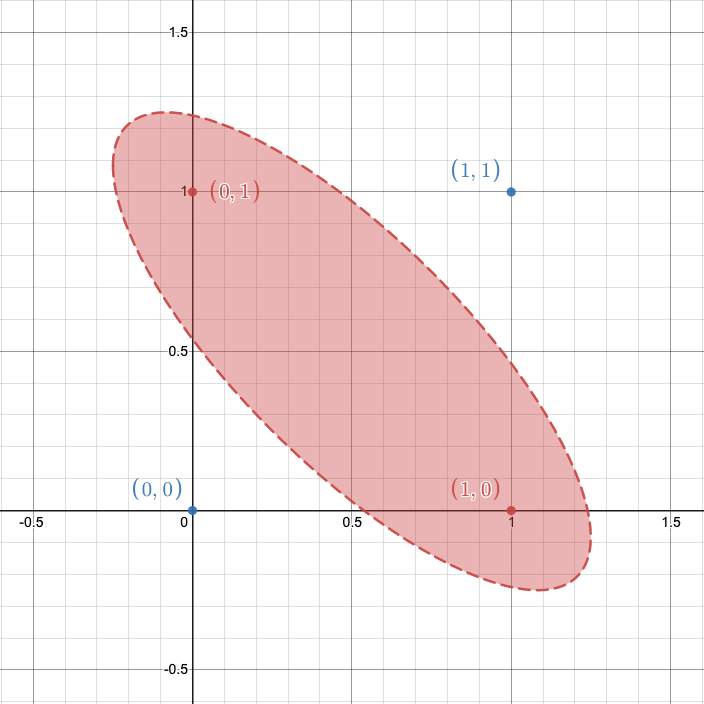
\includegraphics[scale=0.35]{Ellipse}
        \end{center}
\end{enumerate}
\end{proof}



% -------------------------
% Question 2
% -------------------------
\hrule
\bigskip

\begin{proof}[\color{red}{\textbf{Problem 2}: Name}]

\hfill

\begin{enumerate}[label={\color{blue}{\textbf{2.\arabic*})}}]
    \item 
        text \\
        text \\
        text 
        
        
    \item 
        text \\
        text \\
        text 
        
        
    \item 
        text \\
        text \\
        text 
    
\end{enumerate}
\end{proof}
% -------------------------
% Question 3
% -------------------------
\hrule
\bigskip

\begin{proof}[\color{red}{\textbf{Problem 3}: Name}]

\hfill

\begin{enumerate}[label={\color{blue}{\textbf{3.\arabic*})}}]
    \item 
        Two rounds of boosting \\
        \begin{center}
            \begin{tabular}{|l|c|c|}
            \hline
                                & Round 1 & Round 2 \\ \hline
            $\text{weight}_A$              &    $1/6$     &     
            \begin{tabular}{@{}l@{}}
                    = $w_{\text{Round 1}}.e^-{\frac{1}{2}.\ln\frac{1-\epsilon}{\epsilon}$ \\
                    = $w_{\text{Round 1}}.e^-{\frac{1}{2}.\ln\frac{1-(3/6)}{(3/6)}}$ \\
                    = $w_{\text{Round 1}}.e^-{\frac{1}{2}.\ln\frac{1-(3/6)}{(3/6)}}$ \\  
                    = $\frac{1}{2}.\ln{\frac{1 - (1/6)}{(1/6)}}$ \\ 
                    = $\frac{1}{2}.\ln{5}$ \\ 
                \end{tabular}
            \\ \hline
            $\text{weight}_B$              &    $1/6$     &         \\\hline
            $\text{weight}_C$              &    $1/6$     &         \\\hline
            $\text{weight}_D$              &    $1/6$     &         \\\hline
            $\text{weight}_E$              &    $1/6$     &         \\\hline
            $\text{weight}_F$              &    $1/6$     &         \\\hline\hline
            Error rate of h1    &    $3/6$     &         \\\hline
            Error rate of h2    &    $1/6$     &         \\\hline
            Error rate of h3    &    $2/6$     &         \\\hline
            Error rate of h4    &    $3/6$     &         \\\hline
            Error rate of h5    &    $3/6$     &         \\\hline\hline
            weak classifier (h) &   h2  &         \\\hline
            classifier error ($\epsilon$) &    $1/6$     &         \\\hline
            voting power ($\alpha$)        &    
                \begin{tabular}{@{}l@{}}
                    = $\frac{1}{2}.\ln{\frac{1 - \epsilon}{\epsilon}}$ \\  
                    = $\frac{1}{2}.\ln{\frac{1 - (1/6)}{(1/6)}}$ \\ 
                    = $\frac{1}{2}.\ln{5}$ \\ 
                \end{tabular}
            &         \\ \hline
            \end{tabular}
        \end{center}
        
        
    \item 
        \hfill
        \begin{center}
            \begin{tabular}{|l|l|l|l|}
            \hline
            Training Point & \multicolumn{3}{l|}{Classification by ensemble classifier}                                      \\ \hline
            B              & Correctly classified                        & {\color[HTML]{FF0000} \textbf{Misclassified}} & Can't tell \\ \hline
            D              & {\color[HTML]{FF0000} \textbf{Correctly classified}} & Misclassified                        & Can't tell \\ \hline
            F              & Correctly classified                        & {\color[HTML]{FF0000} \textbf{Misclassified}} & Can't tell \\ \hline
            \end{tabular}
        \end{center}
        
        
    \item 
        text \\
        text \\
        text 
    
\end{enumerate}
\end{proof}
\hrule
\bigskip

\end{document}
